\chapter{Введение: распределения, статистики, оценки, гипотезы}

\section{Зачем нужен этот курс}
Практика показывает, что курсов теории вероятности и математической статистики недостаточно для понимания того, как работает случайность и как её модели используются в анализе данных. Наш курс посвящён именно этому - мы изучаем различные применения статистики в анализе данных, попутно знакомясь с более сложными и продвинутыми инструментами. Курс построен от задач, в нём нет сигма-алгебр, разных видов сходимости и есть доказательство ровно одной теоремы, занимающее три строчки.

Методы, которые мы будем изучать, часто баздумно применяются как машины для превращения данных в факты, но они так не работают. Важно понимать границы применимости каждого метода, на этом мы всегда будем подробно останавливаться.

\begin{definition}
Статистика - это наука о том, как по данным делать выводы, поэтому она помогает рационализировать принятие решений и избежать классических когнитивных ловушек (это доказано тоже с помощью статистики!)
\end{definition}

Большинство явлений окружающего мира слишком сложны, чтобы их можно было полностью описать простыми детерминированными закономерностями. Например, мы не можем абсолютно точно предсказывать атмосферные явления, несмотря на то, что понимаем законы, по которым живут отдельные молекулы газов, — в их взаимодействии участвует слишком много факторов, чтобы построить идеальную прогнозирующую модель. Намного более простой процесс — бросание кубиков, но даже его исход мы никогда не можем предугадать (если, конечно, не жульничаем). 

Вместо того, чтобы строить заведомо слишком сложную физическую модель подбрасывания кубика, мы можем сделать шаг назад и представить, что у нас есть некий чёрный ящик, внутреннее устройство которого мы даже не будем пытаться определить. Ящик каким-то образом генерирует случайные события, соответствующие выпадению определённого числа на кубике. Подобные чёрные ящики называются случайными величинами, а выдаваемые ими события~--- реализациями этих случайных величин. Набор реализаций случайной величины называется выборкой из неё. Мы никогда не можем сказать, какое именно событие произойдёт в следующий момент, но, если понаблюдаем за поведением ящика достаточно долго, то начнём замечать некоторые закономерности. Например, если мы честно подбрасываем кубик, то все числа на нём выпадут примерно одинаковое число раз. Именно такие закономерности и являются предметом изучения теории вероятностей и статистики. Если наблюдать за поведением нашего чёрного ящика бесконечно, то каждому событию, которое он генерирует, мы сможем поставить в соответствие вероятность — долю испытаний, завершившихся наступлением этого события. Обратите внимание на то, что эта величина, которой в природе не существует, потому что она определена через бесконечный эксперимент. 

Теория вероятностей изучает модели случайных величин и их свойства. Она позволяет нам понять, какого поведения можно ожидать от чёрного ящика, описанного той или иной моделью, и с какой частотой он будет генерировать интересующие нас события. Статистика  действует в обратном направлении: имея конечные выборки из случайных величин, мы пытаемся сделать выводы об их свойствах и подобрать наиболее подходящие модели, которые позволят нам предсказывать поведение системы в будущих испытаниях. Один из основных инструментов, позволяющих совершать такой переход~--- это закон больших чисел. Он утверждает, что вероятность любого события может быть сколь угодно точно приближена частотой его появления в выборке достаточно большого размера. 

\begin{definition}
    Закон больших чисел~--- на больших выборках частота события хорошо приближает его вероятность.
\end{definition}

\section{Случайная величина}

Случайные величины могут быть дискретными и непрерывными. У дискретных случайных величин счётное множество потенциальных значений, поэтому каждому из них можно поставить в соответствие вероятность с соответствующим номером. Дискретные случайные величины удобно задавать с помощью функции вероятности. С непрерывными случайными величинами это не работает~--- множество их значений имеет мощность континуум, вероятность каждого конкретного значения равна нулю. Поэтому они задаются функциями распределения или плотностями.

Дискретная случайная величина $X$ принимает счётное множество значений
\[
    A = \left\{a_1,a_2,\dots \right\}
\]
с вероятностями $p_1,p_2,\dots$, причем~$\sum\limits_{i}p_1=1$. Для дискретной случайной величины задается \textbf{функция вероятности}:
\[
    f_X\left(a_i\right)=\prob\left(X=a_i\right)=p_i.
\]

Непрерывная же случайная величина задаётся с помощью \textbf{функции распределения}:
\[
F_X(x) = \prob\left(X\leq x\right)
\]
или \textbf{плотности распределения}:
\[
f_X\left(x\right)\colon \int\limits_a^b f_X\!\left(x\right) dx = \prob\left(a\leq X \leq b\right).
\]

\section{Характеристики распределений}
Некоторые характеристики распределений представляют особенный интерес, потому что описывают  важные аспекты поведения случайных величин. Давайте посмотрим на наиболее часто используемые из них.

Матожидание показывает, какое значение наиболее характерно для случайной величины. Дисперсия~--- насколько сильно её значения разбросаны относительно среднего. Ещё одна важная величина~--- квантиль, он определяется для произвольного порядка альфа и представляет собой значение, меньше которого наша случайная величина бывает с вероятностью не меньше альфа, и больше - с вероятностью единица минус альфа.

Есть несколько эквивалентных определений квантиля, например, с разными знаками <>, вас это не должно смущать. Можно определить квантиль через функцию, обратную к функции распределения икс. Квантиль порядка 0.5 - это медиана, центральное значение сл.в., ещё одна характеристика, описывающая среднее. Интерквартильный размах - ещё ожна мера разброса сл.в., так называется потому, что представляет собой разность между 75\% и 25\% квантилями, или квартилями. Наконец, ещё одна характеристика среднего~--- это мода, которая показывает, какое значение сл.в. в каком-то смысле самое популярное. Это максимум либо функции вероятности, либо плотности, в зависимости от того, дискретна случайная величина или непрерывна.


\begin{figure}[!htb]\center
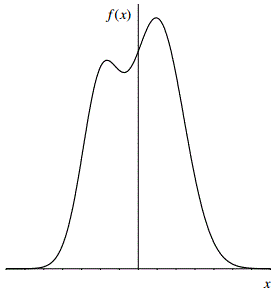
\includegraphics[width=0.7\textwidth]{lectures/lect1/src/Capture.png}
\caption{Пример плотности распределения с нулевым коэффициентом ассиметрии.}
\label{fg:lect1:fig-1}
\end{figure}
Следующая характеристика, коэффициент ассиметрии
\[
\gamma_1 = \mathbb{E} \left( \frac{X-\mathbb{E}X} {\sqrt{\mathbb{D}X}} \right)^3,
\]
третий центральный момент, показывает, в какую сторону распределение скошено. Если он положителен, значит, что у распределения левый хвост больше, если отрицателен~--- правый. Важно, что равенство коэффициента ассиметрии нулю - необходимое, но не достаточное условие симметричности распределения. На картинке~\ref{fg:lect1:fig-1} пример плотности распределения с нулевым коэффициентом ассиметрии.


\begin{figure}[!htb]\center
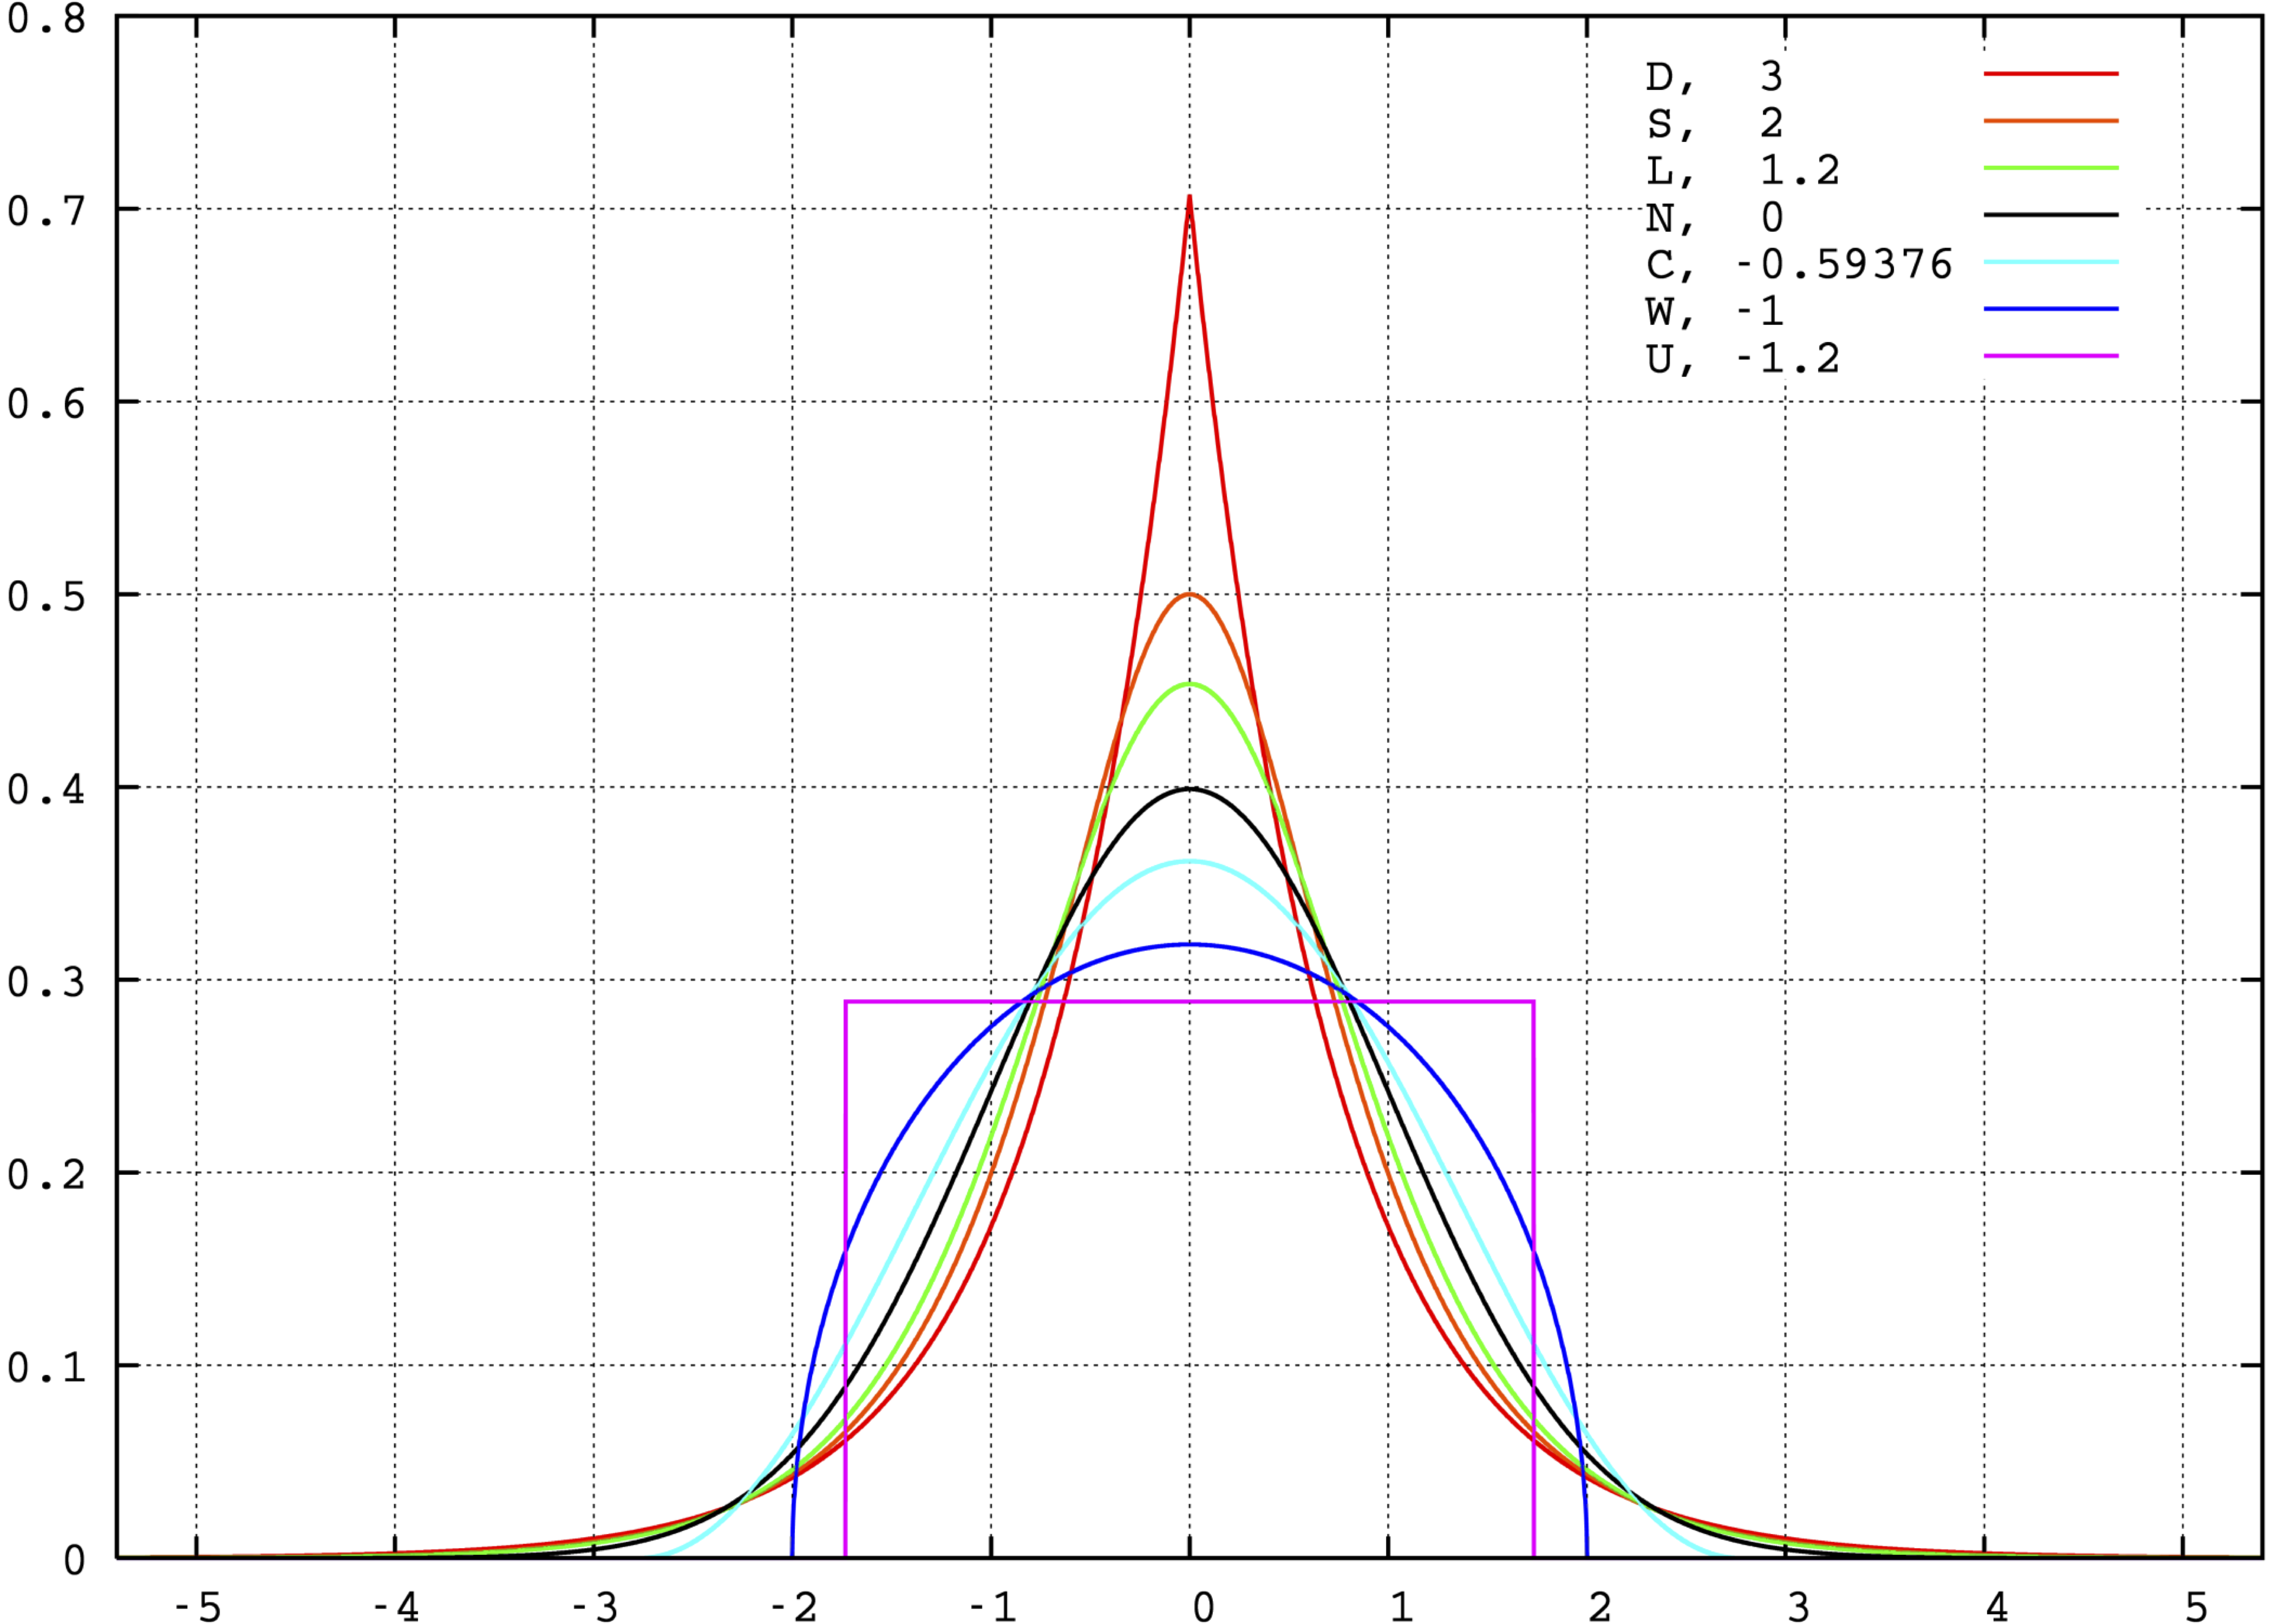
\includegraphics[width=0.7\textwidth]{lectures/lect1/src/kurtosis.png}
\caption{Пример плотностей распределения с различными коэффициентами эксцесса.}
\label{fg:lect1:fig-2}
\end{figure}
Коэффициент эксцесса~--- четвёртый центральный момент
\[
    \gamma_2 =  \frac{\mathbb{E}\left(X-\mathbb{E}X\right)^4}{\left(\mathbb{D}X\right)^2} - 3,
\]
это мера того, насколько тяжелы хвосты распределения. Тройка здесь вычитается для того, чтобы распределения было удобно сравнивать с нормальным: получается, что у распределений с более тяжёлыми хвостами, чем у нормального (например, у распределения Стьюдента), коэффициент эксцесса положительный, а у более компактных распределений~--- отрицательный. Подробнее можно увидеть на рис.~\ref{fg:lect1:fig-2} на примере равномерного распределения.


\section{Основные распределения}
\paragraph{Нормальное распределение}
\begin{figure}[!htb]\center
 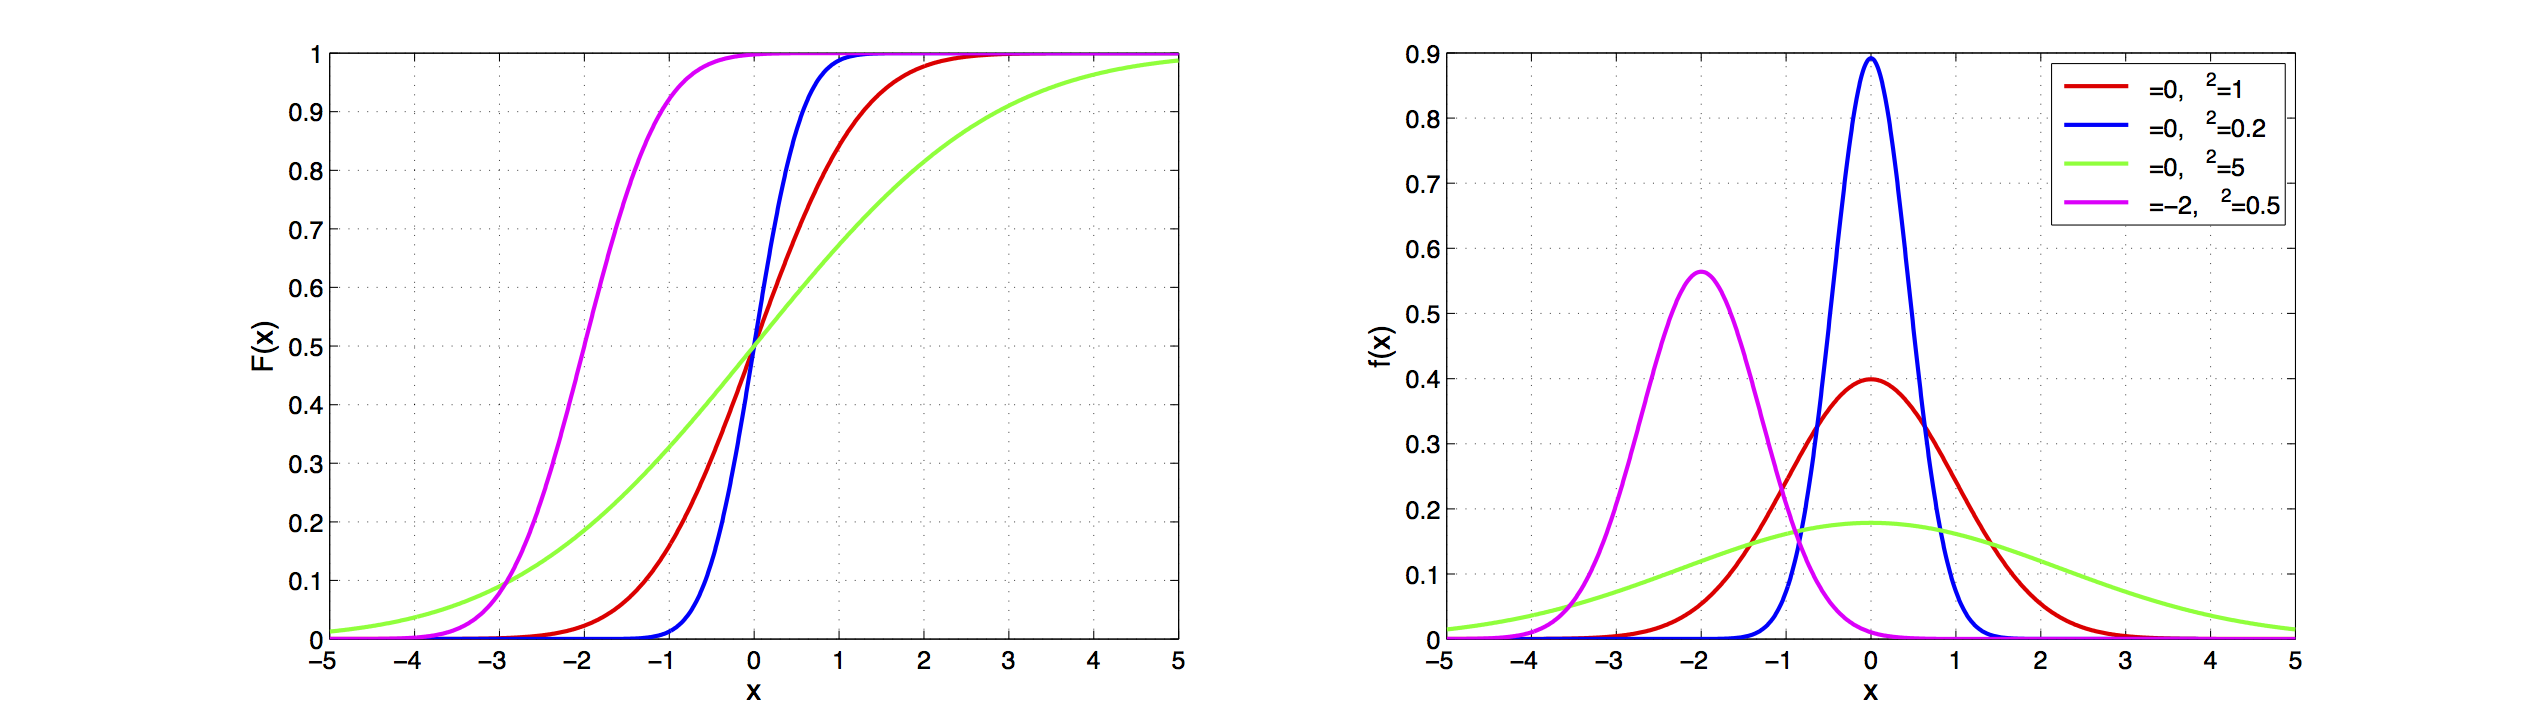
\includegraphics[width=\textwidth]{lectures/lect1/src/norm.png}
\caption{Функции и плотности распределений нормальной слуйчайной величины.}
\label{fg:lect1:fig-3}
\end{figure}
Функция нормального распределения определяется через интеграл ошибок
\begin{align*}
     F\left(x\right) &= \Phi\left(\frac{x-\mu}{\sigma}\right)                &\Phi\left(x\right) &= \frac1{\sqrt{2\pi}} \int_{-\infty}^x e^{-\frac{t^2}{2}} dt\\
     f\left(x\right) &= \frac1{\sigma}\phi\left(\frac{x-\mu}{\sigma}\right)  &\phi\left(x\right) &= \frac1{\sqrt{2\pi}} e^{-\frac{x^2}{2}},
\end{align*}
который в аналитическом виде не берётся. Многие непрерывные распределения, которыми мы будем пользоваться, определяются через подобные интегралы. Главное, что все значения функций можно определить численно. Нормальное распределение с нулевым средним и единичной дисперсией называется стандартным нормальным. 

Распределение выборочного среднего из центральной предельной теоремы достаточно хорошо описывается нормальным, если количество усредняемых случайных достаточно велико и их распределение не слишком скошено. Достаточно велико на практике значит~$>30$.

\paragraph{Распределение хи-квадрат}
Хи-квадрат с~$k$ степенями свободы~--- это распределение суммы квадратов~$k$ независимых стандартных нормальных случайных величин:
\[
    \sum\limits_{i=1}^k X_i^2 \sim \chi^2_k.
\]
Благодаря тому, что функция распределения и плотность задаются через гамма-функции, мы можем использовать хи-квадрат и с нецелым числом степеней свободы.


\begin{figure}[!htb]\center
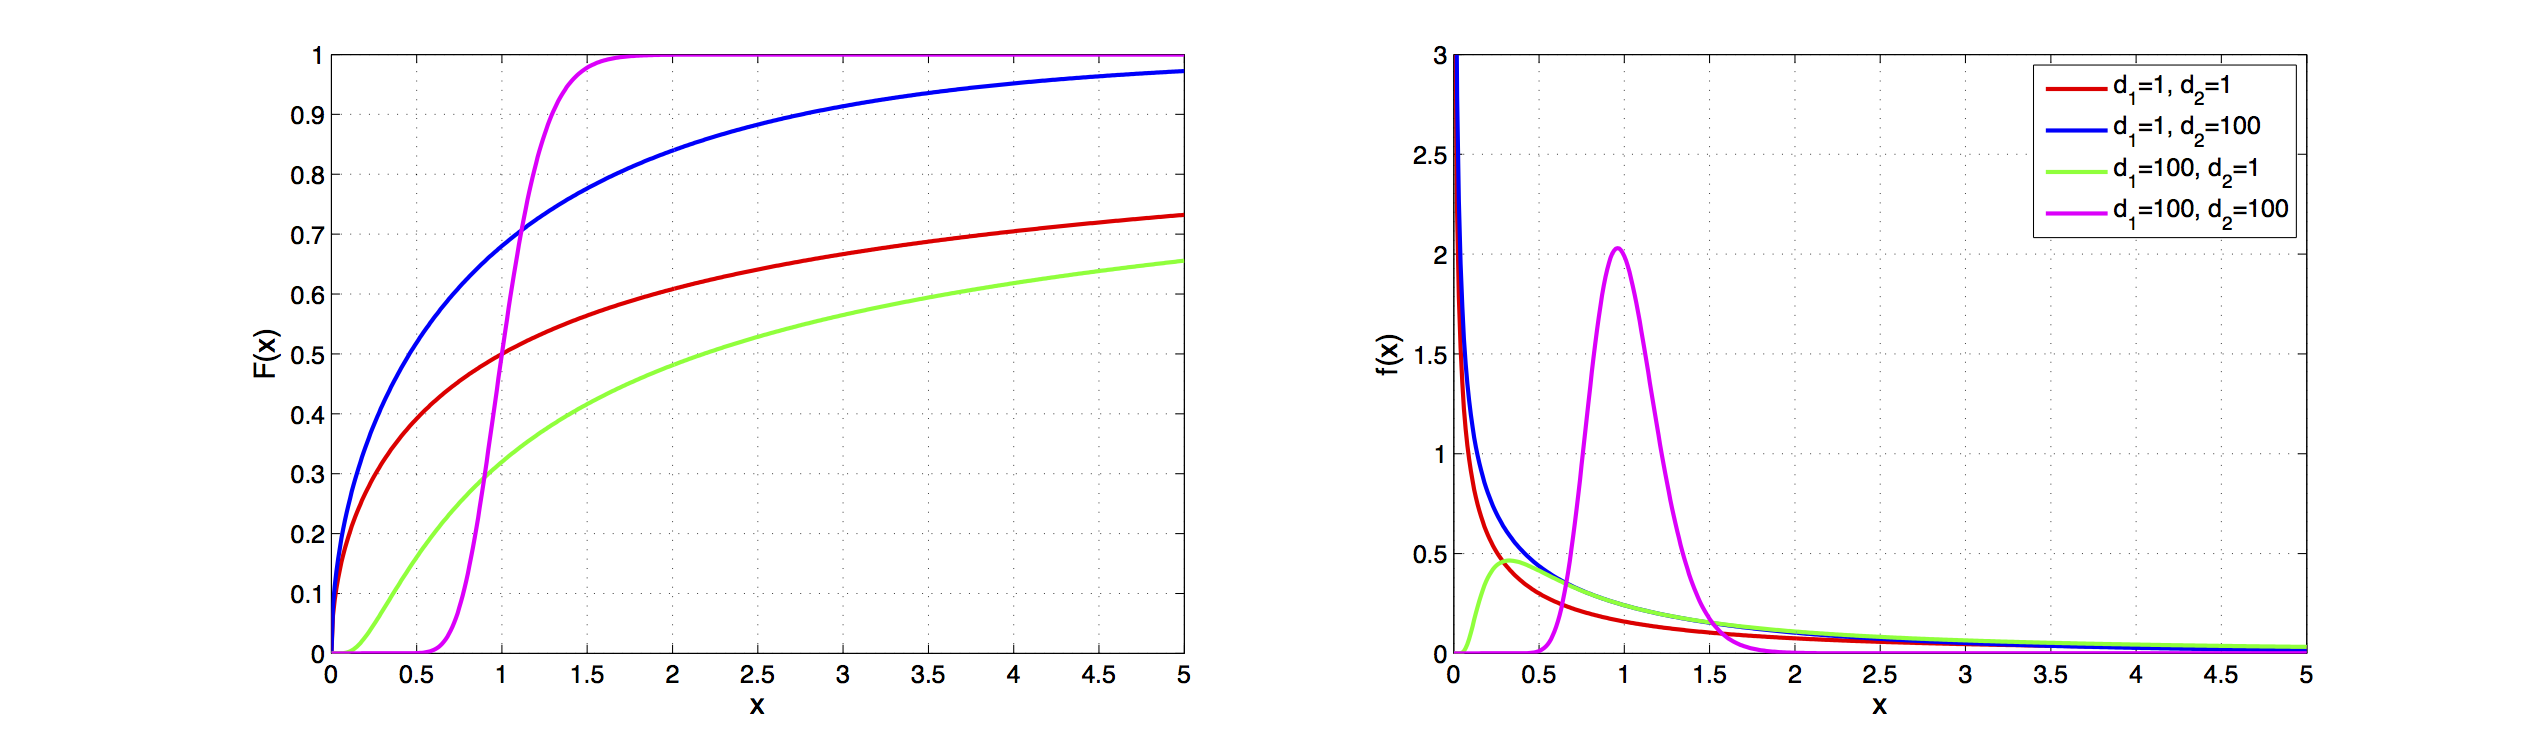
\includegraphics[width=0.7\textwidth]{lectures/lect1/src/fish.png}
\caption{Пример плотности распределения с нулевым коэффициентом ассиметрии.}
\label{fg:lect1:fig-4}
\end{figure}
\paragraph{Распределение Фишера} Распределение Фишера может выглядеть очень по-разному при разных значениях своих параметров. На рис.~\ref{fg:lect1:fig-4} показаны различные вариации распределения ФИшера взависимости от параметров.

\paragraph{Распределение Стьюдента} Распределение Стьюдента похоже на стандартное нормальное - у него всегда нулевое среднее, но хвосты более тяжёлые. Чем больше число степеней свободы, тем меньше отличия - уже начиная с~$\nu=30$ визуально отличить из невозможно. Как и предыдущие, может определяться с нецелым числом степеней свободы - мы будем этим активно пользоваться в дальнейшем.

\paragraph{Распределение Бернулли} TODO

\paragraph{Биномиальное распределение} TODO

\paragraph{Распределение Пуассона} Распределение Пуассона является часто встречающимся распределение для счётчиков, точно так же как нормальное - для непрерывных случайных величин. Это не значит, что все счётчики описываются этим распределением, а только что его имеет смысл попробовать в первую очередь. Часто используется для задачи где нужно распределение числа независимых событий в фиксированном временном или пространственном интервале.

\section{Статистика}

Основной задачей статистики является описание $F_X(x)$ по реализации выборки~$X^n$. Выборка $X^n$ называется простой, если~$X_1,\dots,X_n$~--- независимые одинаково распределённые случайные величины (i.i.d.).

\begin{definition}
    Генеральная совокупность~--- множество объектов, свойства которых подлежат изучению в рассматриваемой задаче.
\end{definition}

\begin{definition}
    Выборка~--- конечное множество объектов, отобранных из генеральной совокупности для проведения измерений.
    \[
        X^n=\left(X_1,\dots,X_n\right),
    \]
    где $n$~--- объём выборки.
\end{definition}


\begin{figure}[!htb]\center
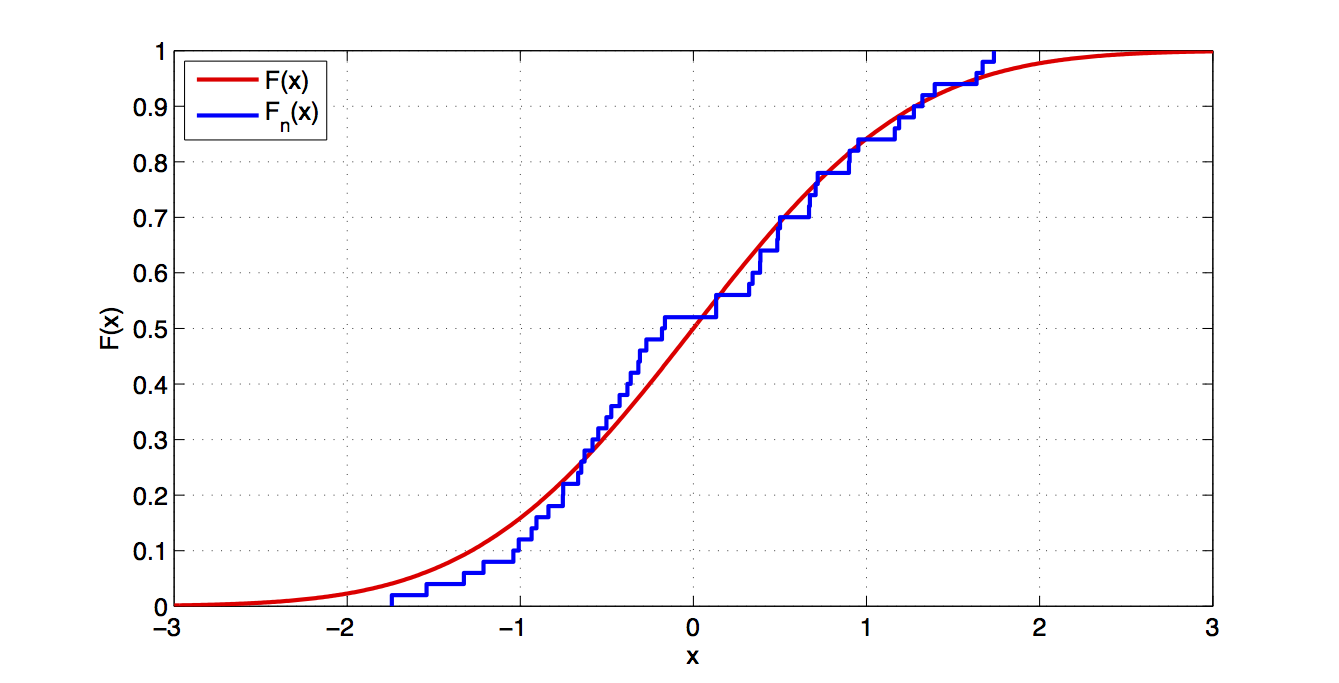
\includegraphics[width=0.9\textwidth]{lectures/lect1/src/ecdf.png}
\caption{Эмпирическая функция распределения по выборке из 50 объектов.}
\label{fg:lect1:fig-5}
\end{figure}
Одним из способов приблизить по выборке функцию распределения является эмпирическая функция распределения:
\[
    F_n\left(x\right) = \frac1{n} \sum\limits_{i=1}^n \left[X_i\leq x\right].
\]
На картинке~\ref{fg:lect1:fig-5} эмп. функция распределения построена по выборке объёма~$50$ из стандартного нормального распределения.

\begin{figure}[!htb]\center
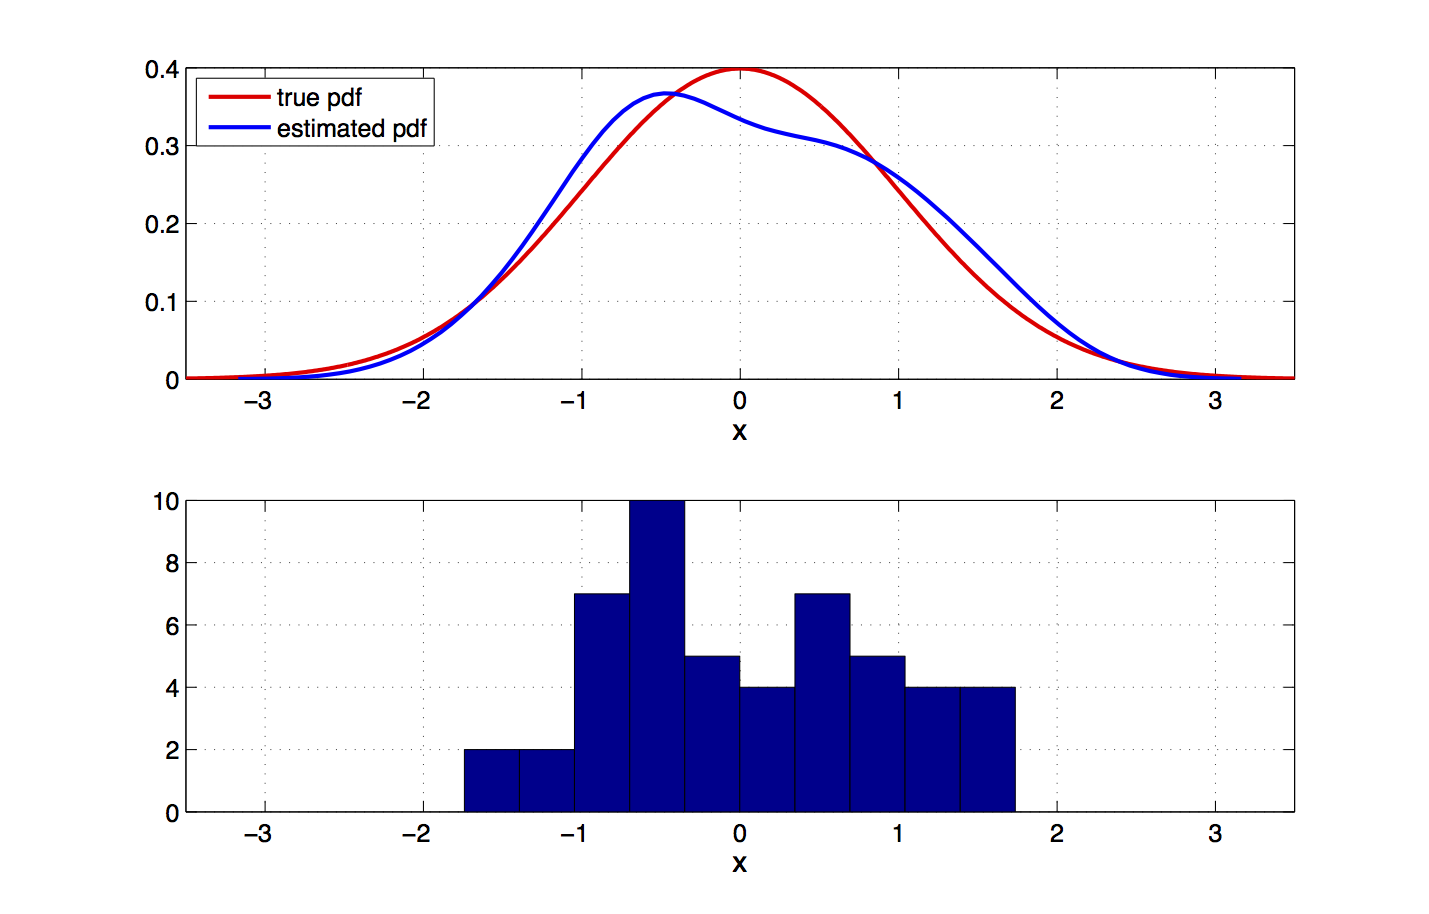
\includegraphics[width=0.9\textwidth]{lectures/lect1/src/epdf.png}
\caption{Пример ядерной оценки функции плотности и гистограммы.}
\label{fg:lect1:fig-6}
\end{figure}
Если же мы хотим приблизить не функцию распределения, а плотность, есть два способа - гладкая оценка плотности, которая строится с помощью ядерного сглаживания, и гистограмма. На картинке построены по той же самой выборке, что и на предыдущем слайде. Оба метода имеют скрытый параметр - ширина окна сглаживания и число карманов гистограммы; и то, и другое, как правило, выбирается автоматически, но можно этими параметрами манипулировать. Оба способа обладают своими недостатками: гладкая оценка может вылезать за края области определения случайной величины, а гистограмма, как правило, выглядит не очень похоже на исходную плотность. Лучше всего на практике пользоваться обоими способами, которые представлены на рис.~\ref{fg:lect1:fig-6}.

Часто нам интересно не распределение целиком, а какие-то его конкретные характеристики. Самые популярные, естественно, средние. Для оценки таких характеристик мы будем использовать основной инструмент статистики - статистики. 

\begin{definition}
    Статистика $T(X^n)$~--- любая измеримая функция выборки.
\end{definition}

Заметим, что статистикой может быть только измеримая функция, но слово "измеримая" часто упускают. Примеры статистик:
\begin{itemize}
    \item выборочное среднее:
    $$\bar{X} = \frac1{n}\sum\limits_{i=1}^n X_i$$
    \item выборочная дисперсия:
    $$S^2 = \frac1{n-1}\sum\limits_{i=1}^n \left(X_i-\bar{X}\right)^2$$
\end{itemize}

\begin{figure}[!htb]\center
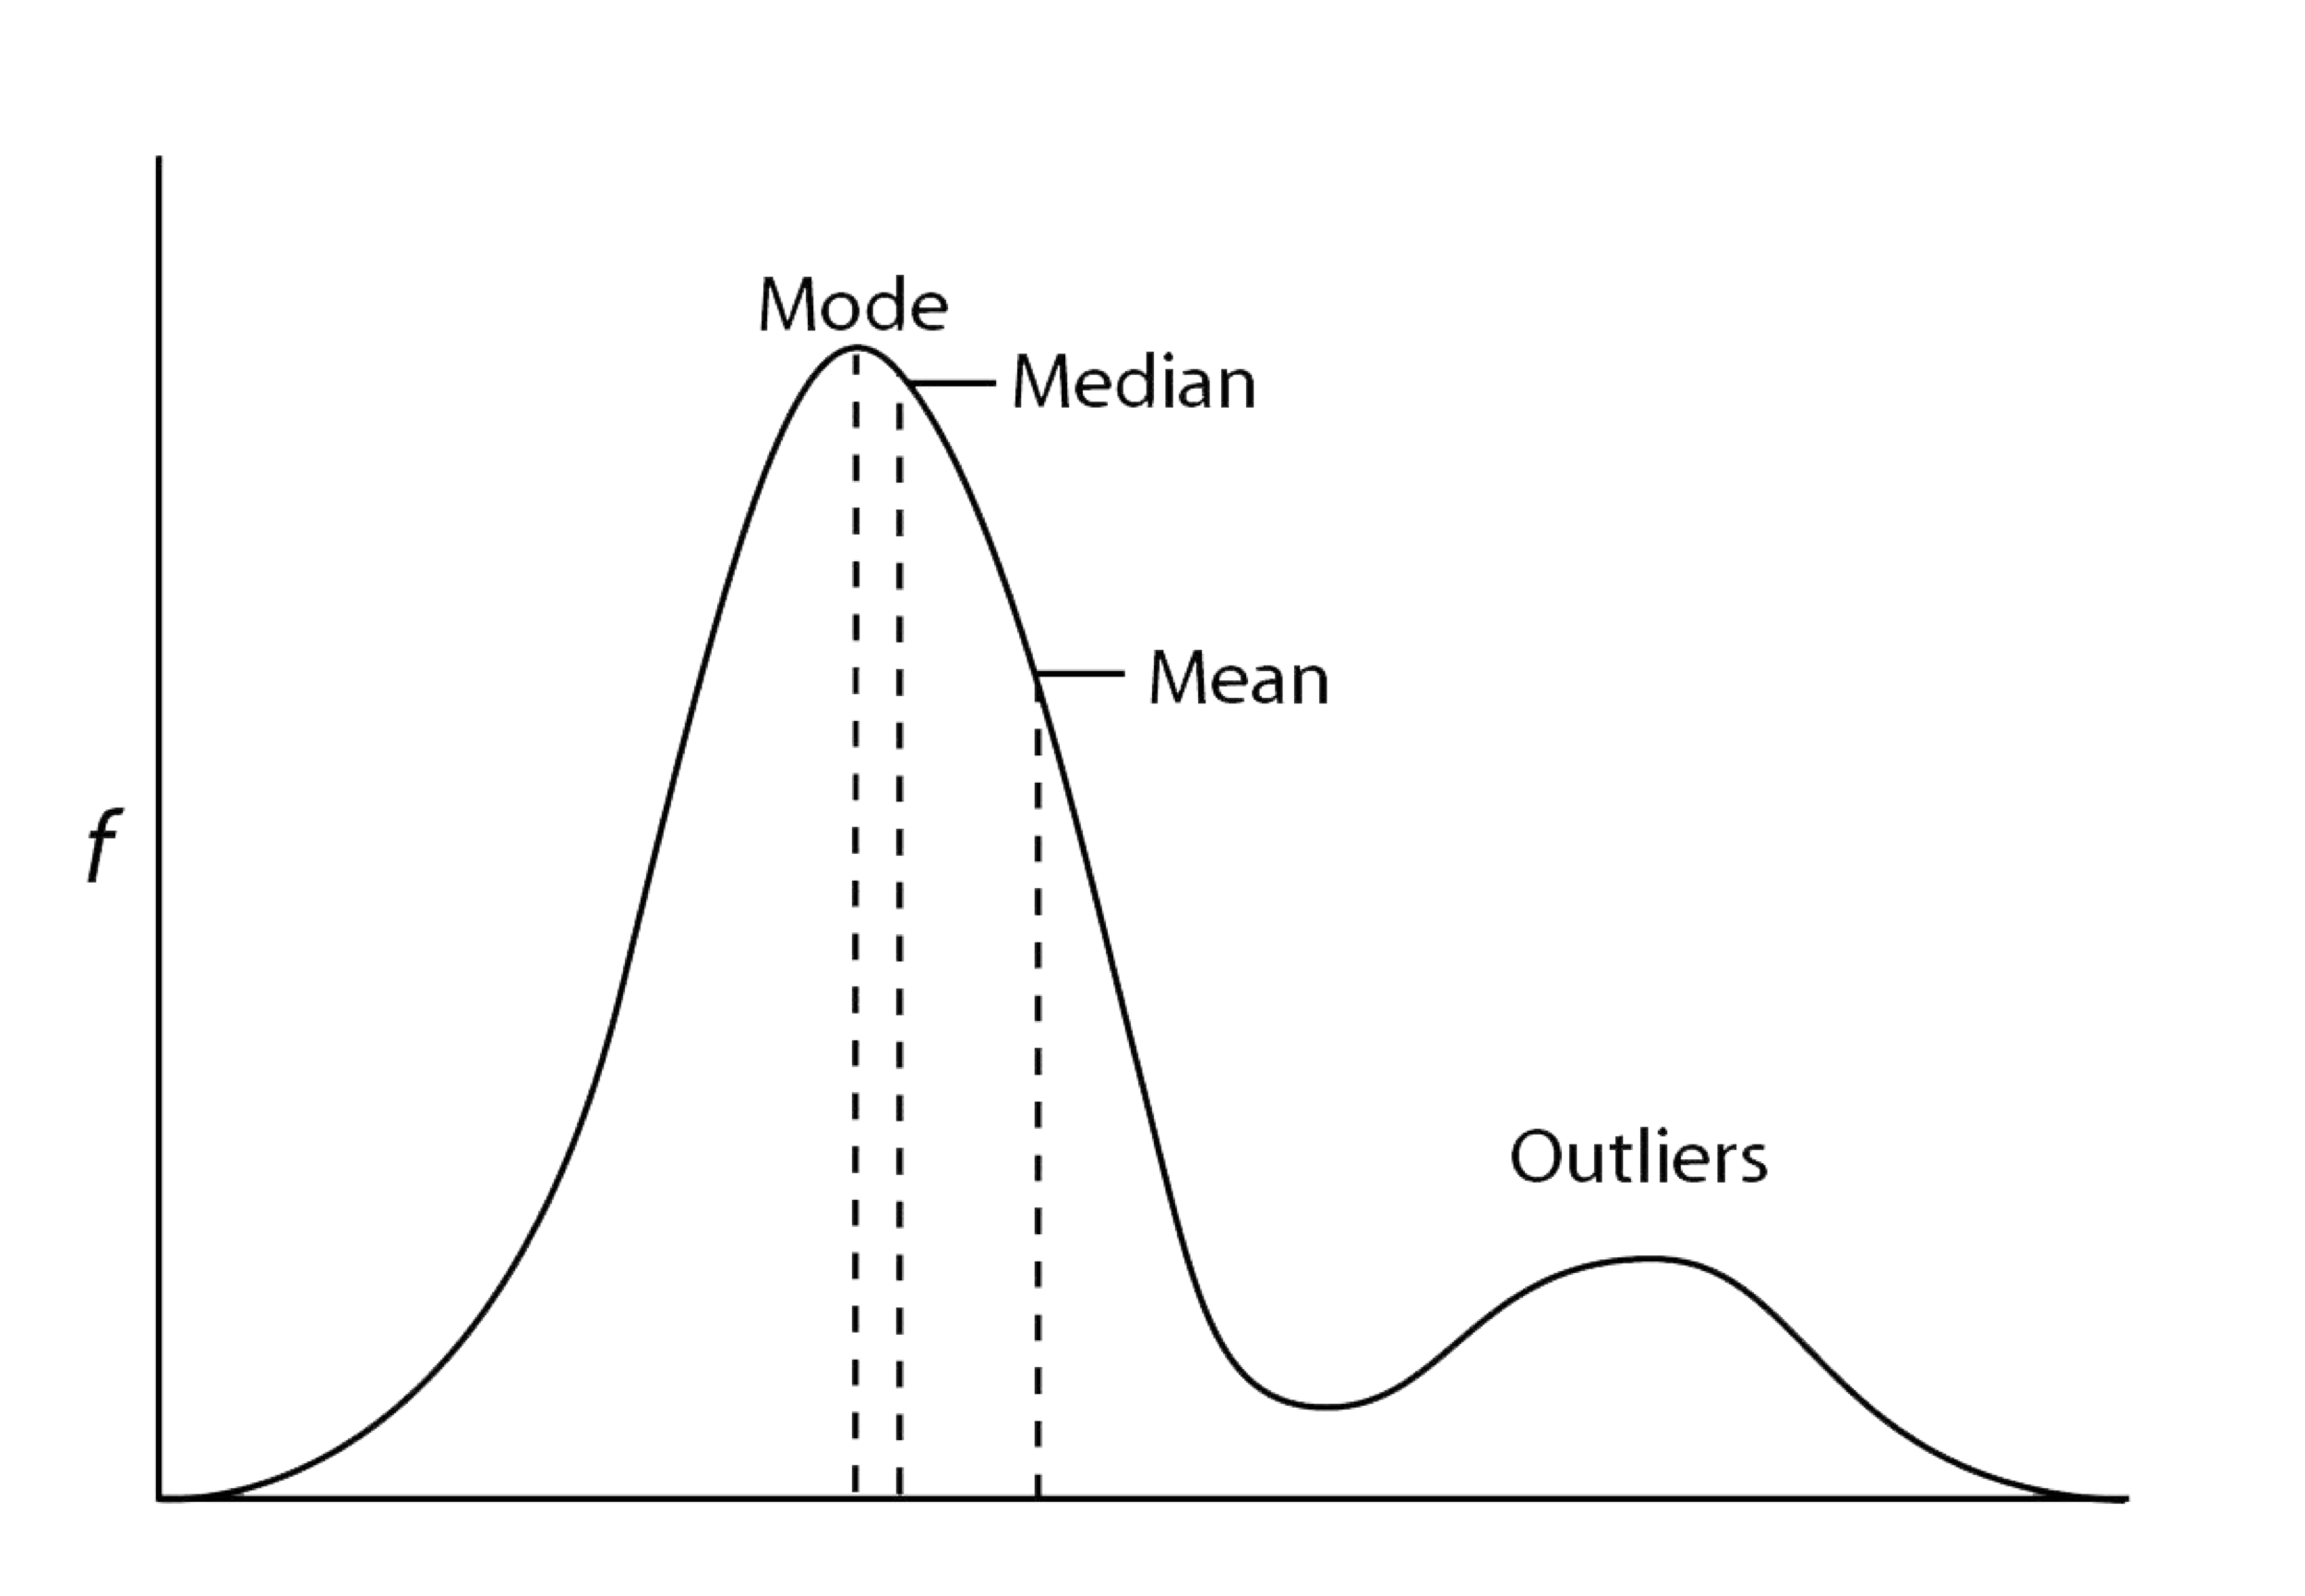
\includegraphics[width=0.7\textwidth]{lectures/lect1/src/mmm.png}
\caption{Пример распределений с разными значениями средних}
\label{fg:lect1:fig-7}
\end{figure}
Средние также бывают разными:
\begin{itemize}
    \item Выборочное среднее~--- среднее арифметическое по выборке.
    \item Выборочная медиана~--- центральный элемент вариационного ряда.
    \item Выборочная мода~--- самое распространённое значение в выборке.
\end{itemize}


\begin{figure}[!htb]\center
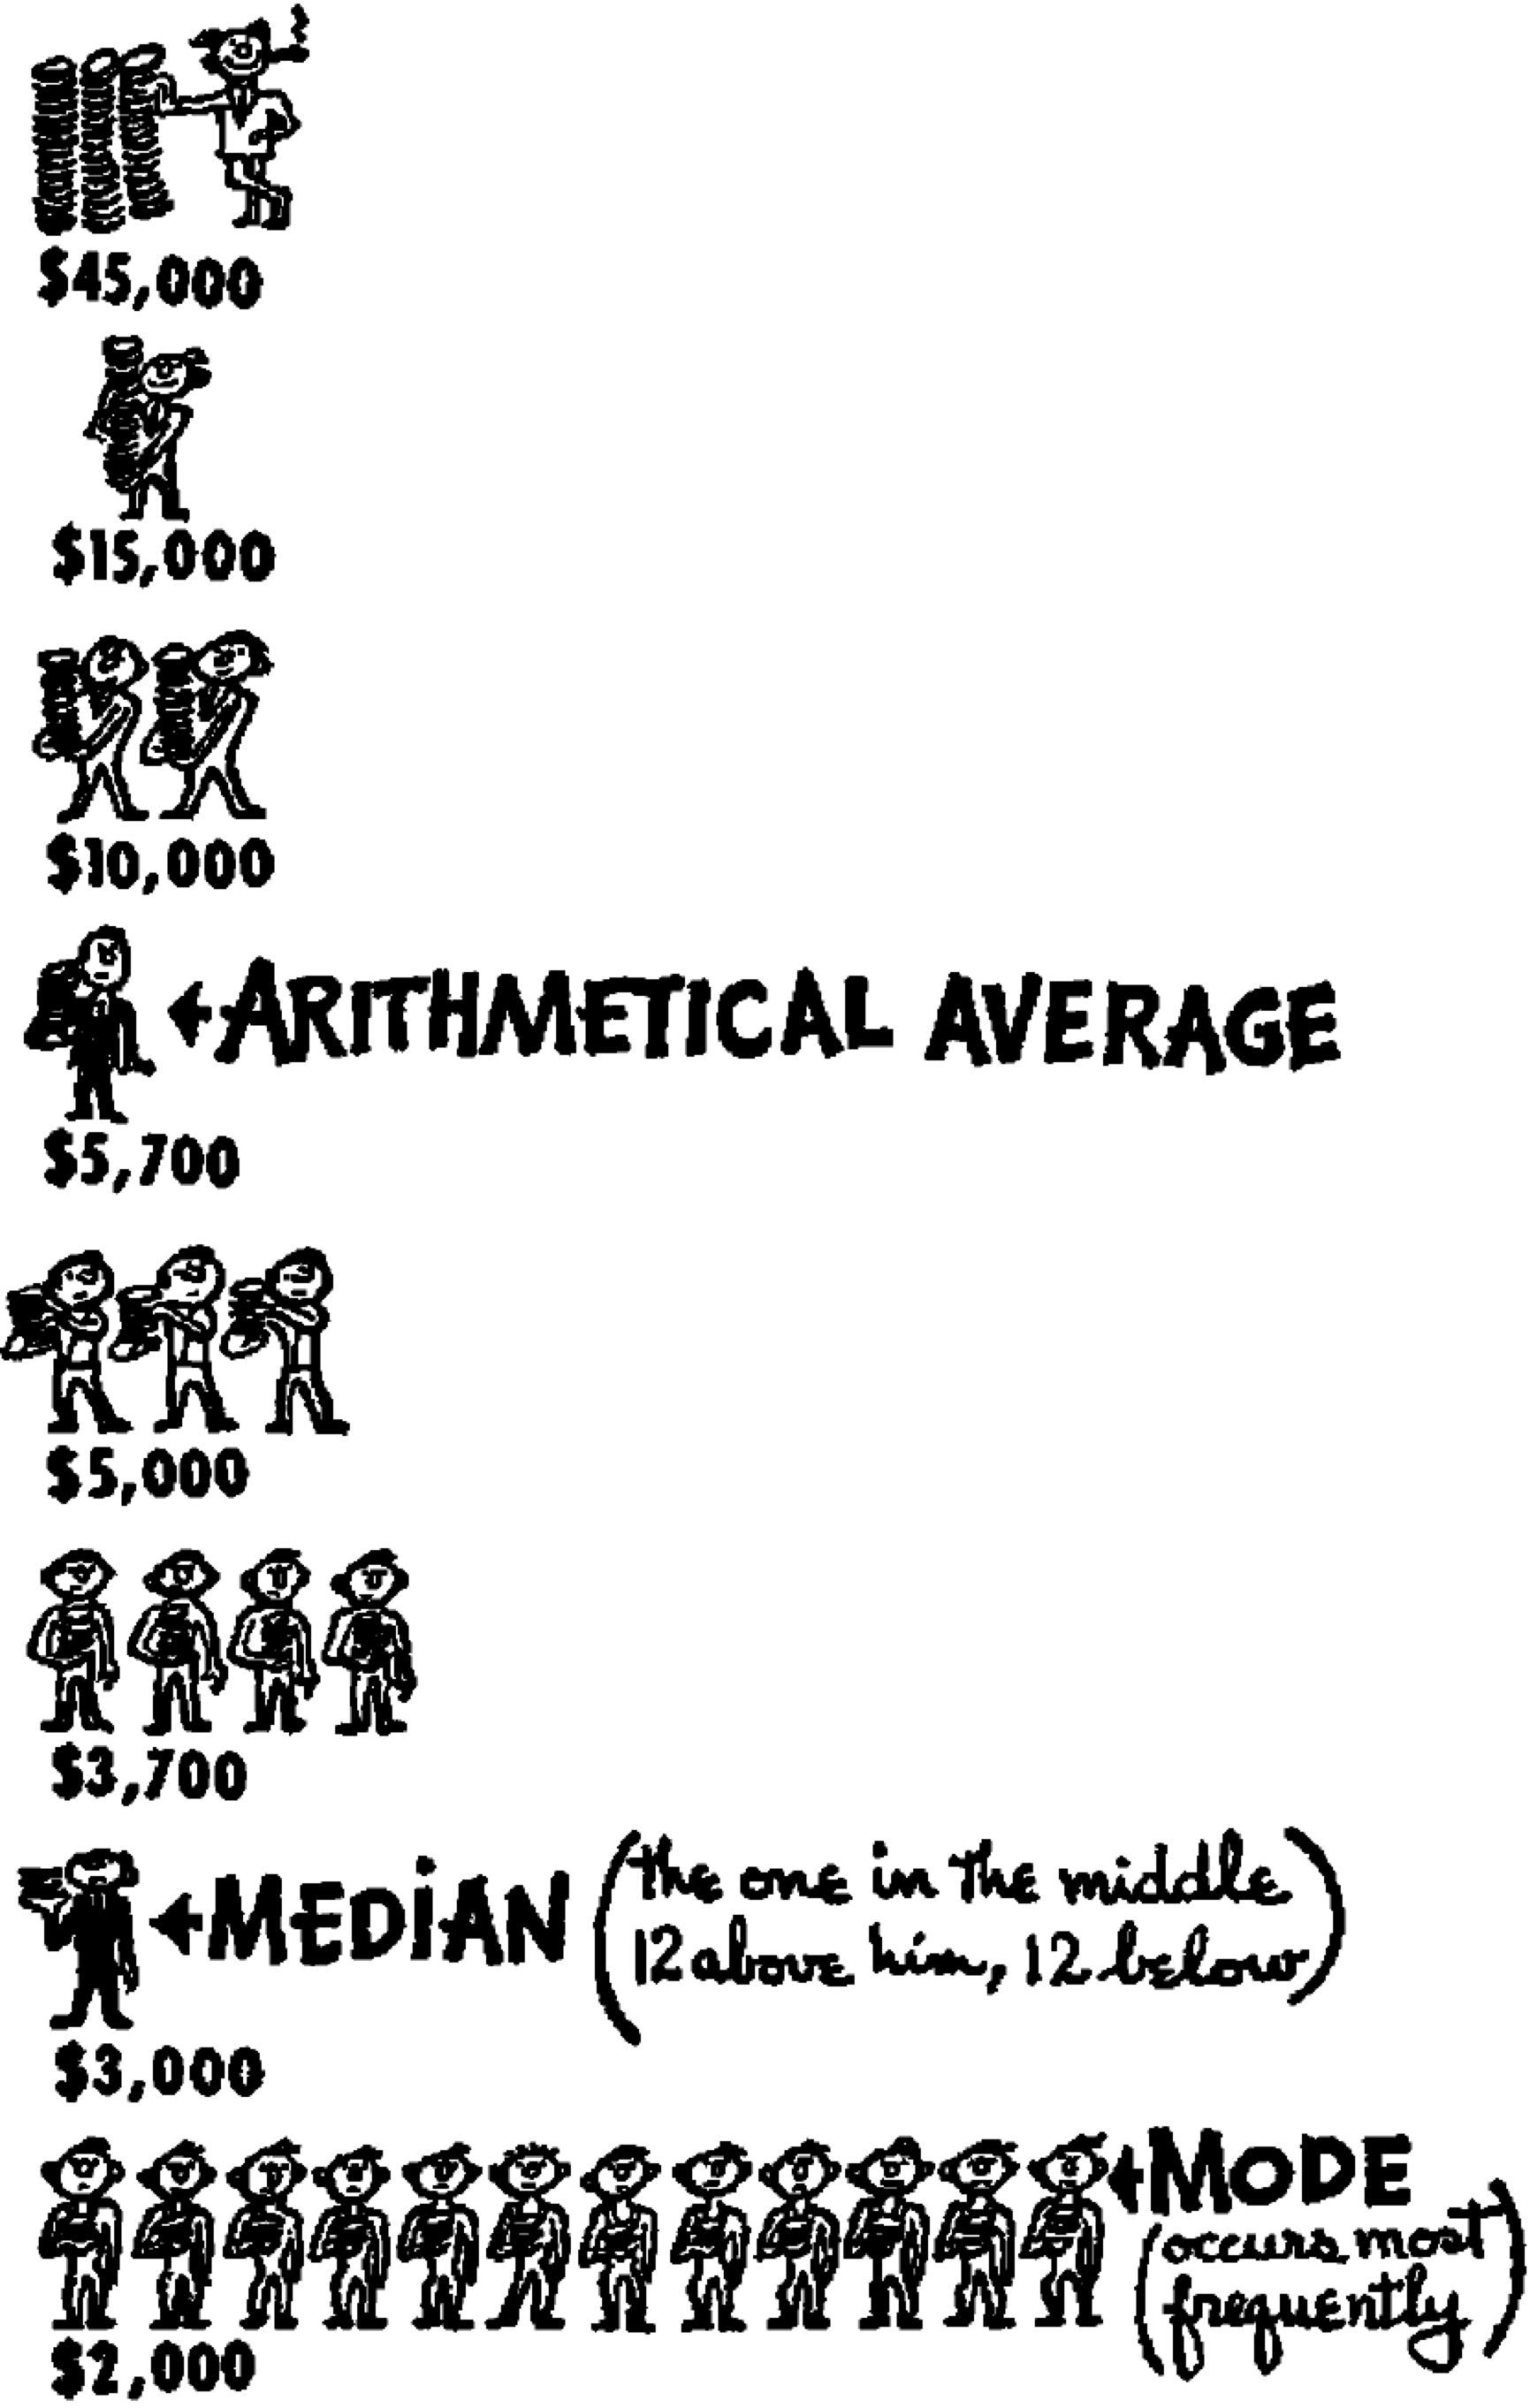
\includegraphics[width=0.3\textwidth]{lectures/lect1/src/howto.png}
\caption{Пример из книги 1954 года ``Как врать с помощью статистики''}
\label{fg:lect1:fig-10}
\end{figure}
Оценки разных средних, как и сами эти разные средние, вовсе не обязаны совпадать, как, например, у распределения на картинке~\ref{fg:lect1:fig-7}. На рис.~\ref{fg:lect1:fig-10} пример из книги 1954 года ``Как врать с помощью статистики''. Дана выборка из~$25$ человек, про которых мы знаем их годовой доход. Представьте, что на основе этих данных нам нужно написать отчёт об уровне дохода в нашей генеральной совокупности, например, стране. Если мы хотим, чтобы отчёт выглядел оптимистично, мы можем написать, что что средний доход составляет 5700\$. Если нам нужны более пессимистичные оценки, мы можем написать, что большая часть людей получает 2000\$; ну и промежуточный вариант со средним доходом 3000\$. Все эти оценки являются оценками разных средних, и часто упоминание того, какое именно среднее было использовано, из текста выбрасывается. Мы рассказываем вам это не для того, чтобы вы так делали, а чтобы вы понимали, что другие люди могут так делать.

\begin{figure}[!htb]\center
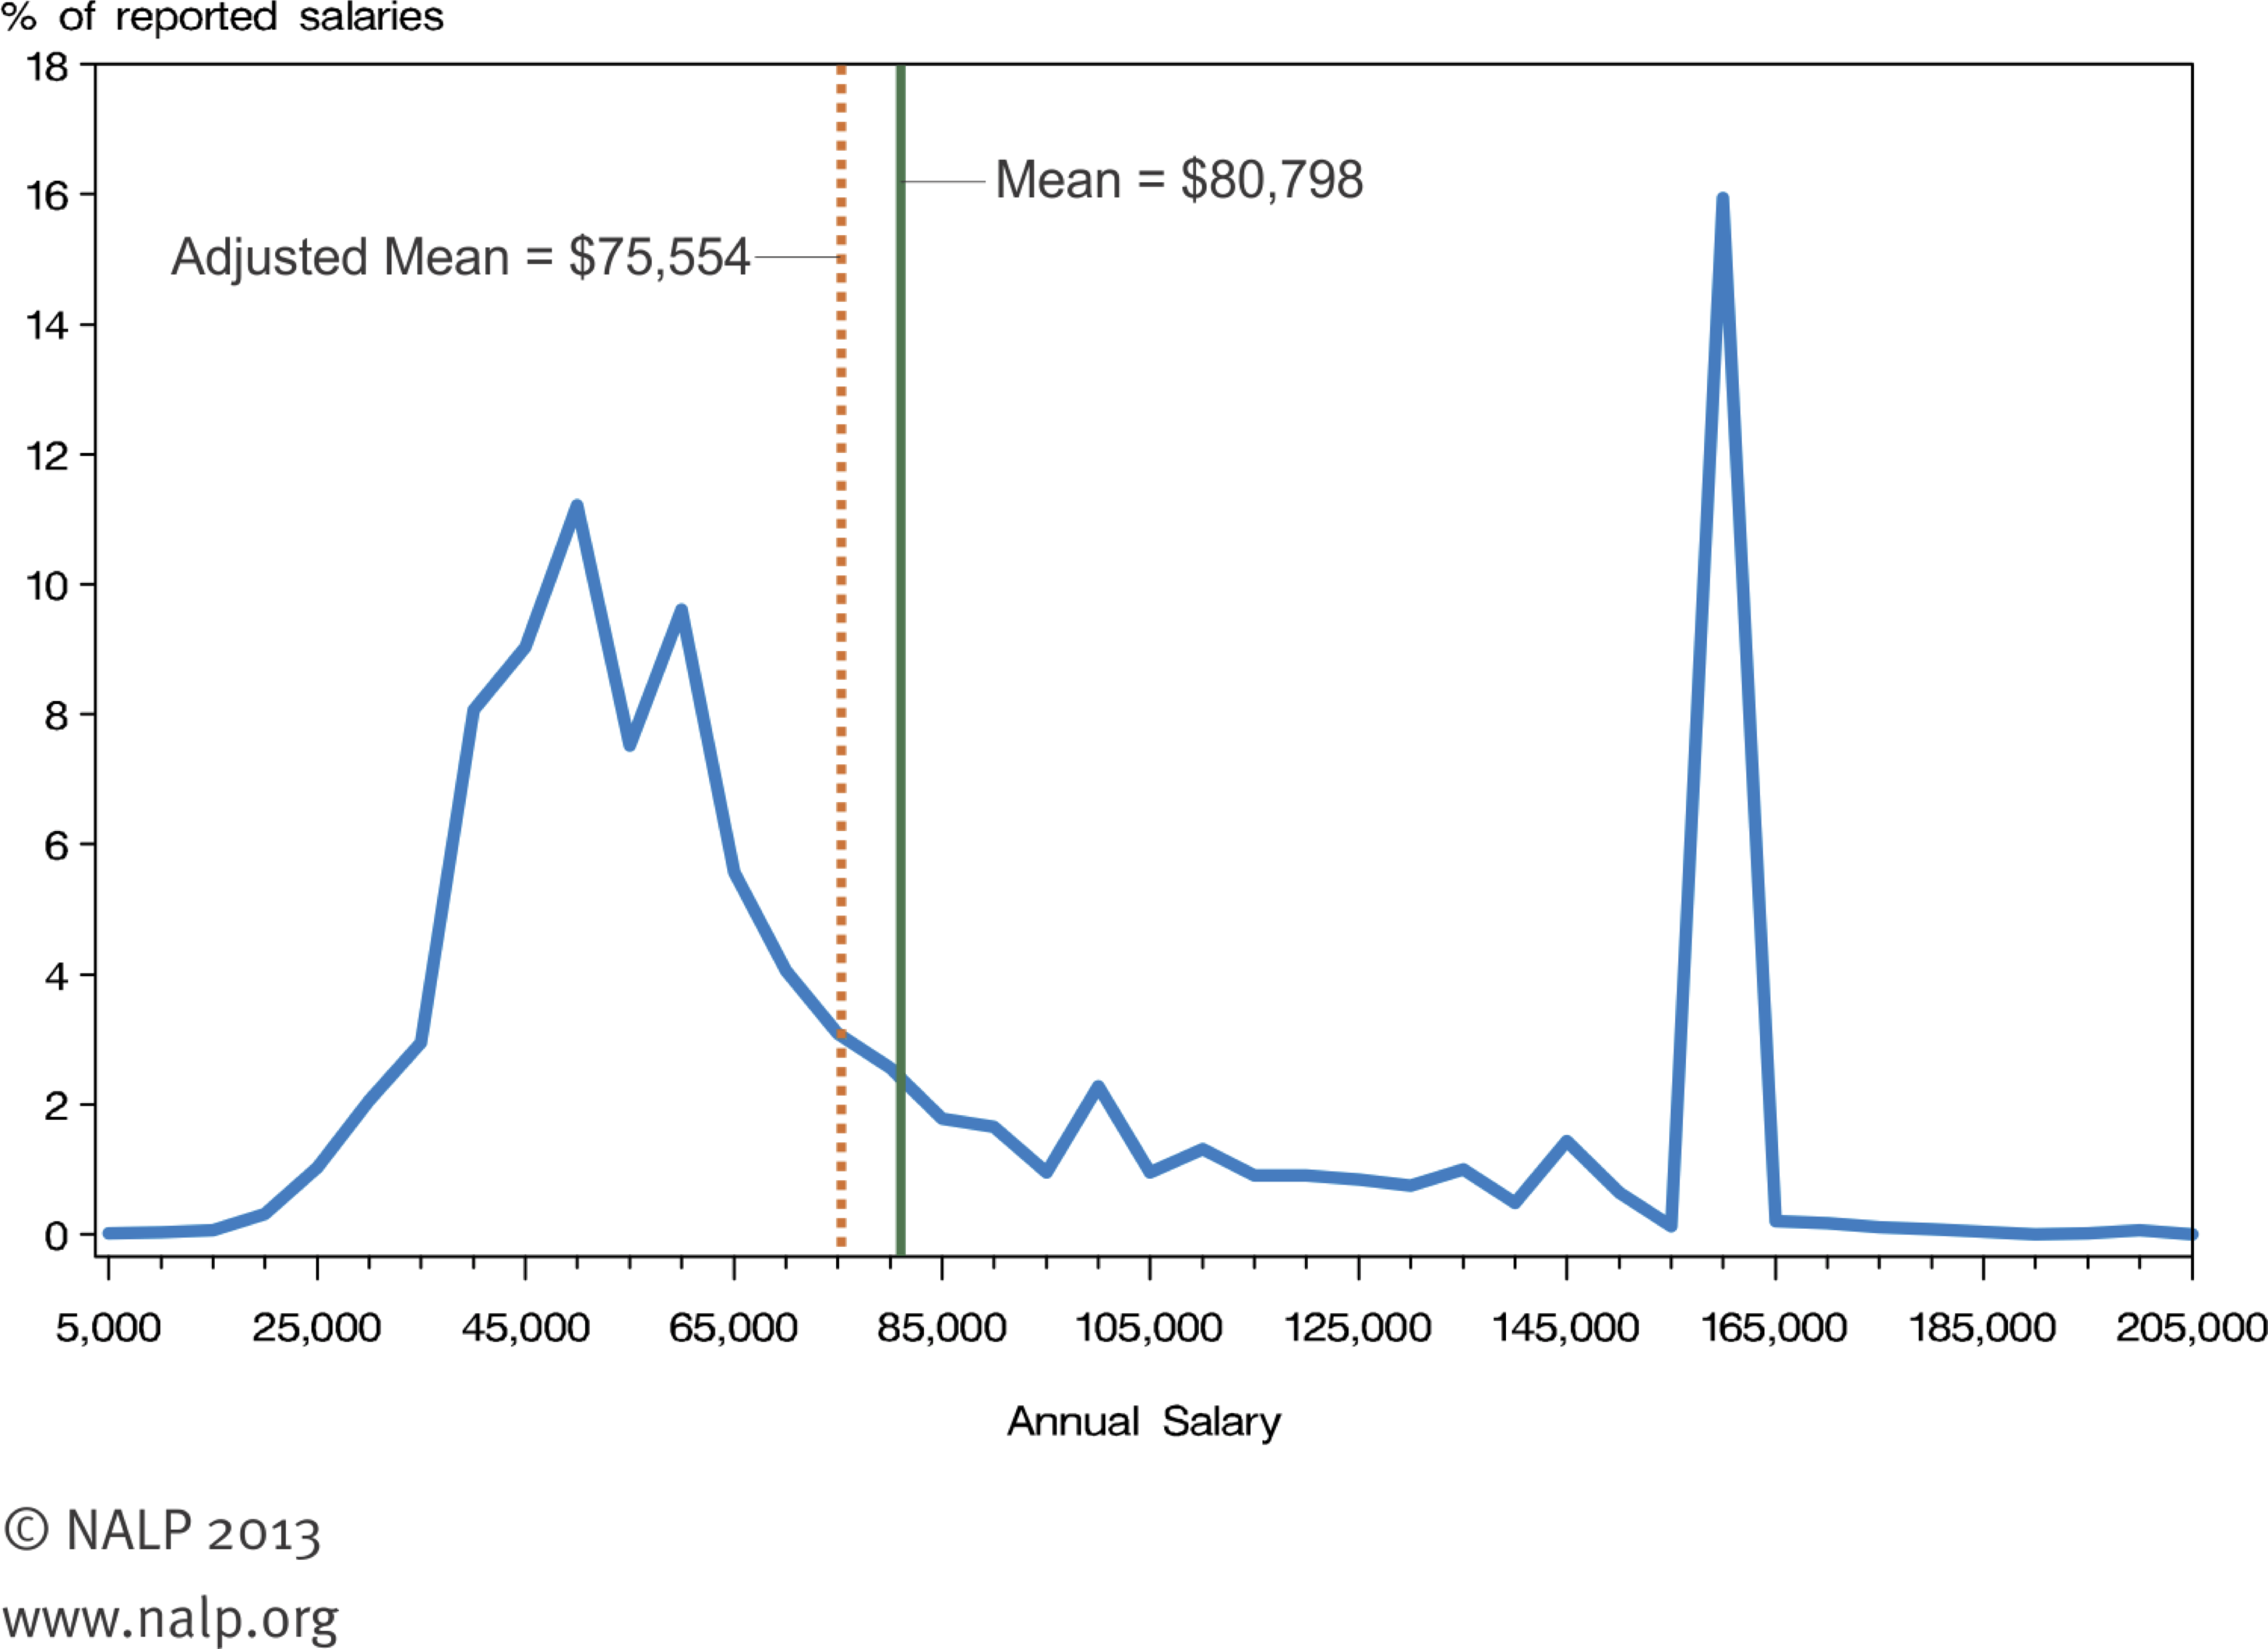
\includegraphics[width=0.9\textwidth]{lectures/lect1/src/nalp2012.png}
\caption{Уровень стартовой заработной платы выпускников юридических факультетов, США, 2012, данные NALP.}
\label{fg:lect1:fig-8}
\end{figure}
Вообще говоря, никакое среднее не может полностью передать распределение исследуемой вами величины. Пример - стартовые заработные платы выпускников юридических факультетов по данным опроса участников американской ассоциации юристов. Их средняя зарплата составляет 80000, но по картинке~\ref{fg:lect1:fig-8}, которая представляет собой по сути выборочную оценку плотности распределения показателя, хорошо видно, что 80000\$ не получает примерно никто. Как бы вы не посчитали по этим данным среднее, глядя на него, а не на картинку, вы никогда не поймёте, как устроены ваши данные.

\begin{figure}[!htb]\center
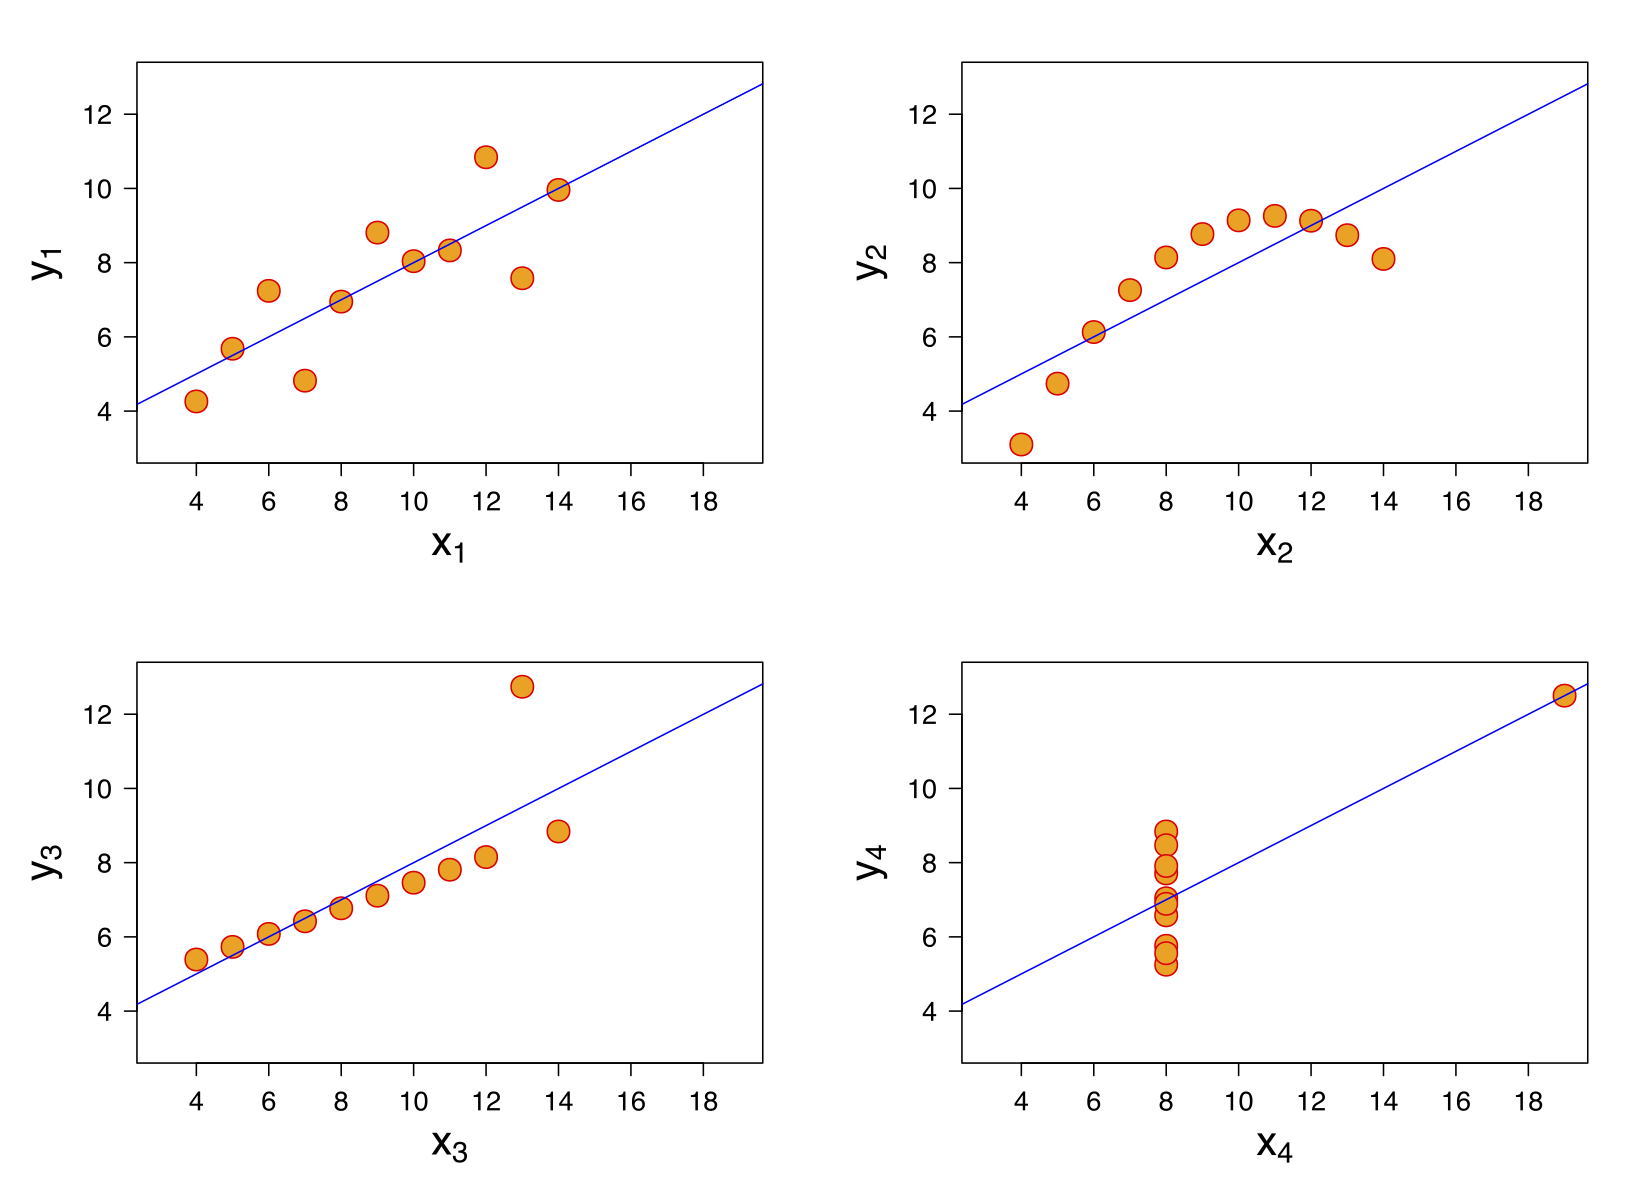
\includegraphics[width=0.9\textwidth]{lectures/lect1/src/Anscombe's_quartet.png}
\caption{Квартет Энскомба}
\label{fg:lect1:fig-9}
\end{figure}

Это справедливо, разумеется, не только для средних. Один из самых известных примеров - это квартет Энскомба, четыре пары таких выборок, что их выборочные средние, дисперсии и корреляции совпадают с точностью до двух знаков после запятой. Таблица~\ref{tg:lect1:fig-9} показывает нам, что все четыре пары выборок примерно одинаковые, но, если мы посмотрим, как они выглядят на графиках~\ref{fg:lect1:fig-9}, мы увидим, что это далеко не так. Мораль: не полагайтесь на обобщающие статистики, всегда смотрите на оценки плотности и гистограммы, чтобы понять, как именно ваши данные устроены.

\begin{table}[!htb]
    \centering
    \begin{tabular}{|l|cccc|}
        \hline
        \text{№}& 1    & 2    & 3    & 4    \\ \hline
        $\bar{x}$ & 9    & 9    & 9    & 9    \\ \hline
        $S_x$   & 11   & 11   & 11   & 11   \\ \hline
        $\bar{y}$ & 7.5  & 7.5  & 7.5  & 7.5  \\ \hline
        $S_y$    & 4.127& 4.127& 4.128& 4.128\\ \hline
        $r_{xy}$  & 0.816& 0.816& 0.816& 0.816\\ \hline
    \end{tabular}
    \caption{Квартет Энскомба}
    \label{tg:lect1:fig-9}
\end{table}

\section{Оценки}

Пусть распределение генеральной совокупности параметрическое:
\[
F(x) = F(x,\theta).
\]

Статистика $\hat{\theta}_n = \hat{\theta}\left(X^n\right)$~--- точечная оценка параметра $\theta$.

Чтобы выбрать оценку требуется рассмотреть различные характеристики статистики:
\begin{enumerate}
    \item \textbf{Состоятельность:} $\plim\limits_{n\rightarrow\infty} \hat{\theta}_n  = \theta$.
    \item \textbf{Несмещённость:} $\mathbb{E}\hat{\theta}_n = \theta$.
    \item \textbf{Асимптотическая несмещённость:} $\lim\limits_{n\rightarrow\infty}\mathbb{E}\hat{\theta}_n = \theta$.
    \item \textbf{Оптимальность:} $\mathbb{D}\hat{\theta}_n = \min\limits_{\hat{\theta}\colon \mathbb{E}\hat{\theta}=\theta} \mathbb{D}\hat{\theta}$.
    \item \textbf{Робастность:} устойчивость $\hat{\theta}_n$ относительно 
        \begin{itemize}
            \item отклонений истинного распределения $X$ от модельного семейства
            \item выбросов, содержащихся в выборке
        \end{itemize}
\end{enumerate}

Определение робастности вообще говоря не является строгим, потому что "отклонение" и "выброс" также строго не определяются.


Популярным методом получения точечных оценок является метод максимального правдоподобия (ММП). ММП - популярный метод получения оценок, когда семейства распределений заданы с точностью до параметров:
\begin{align*}
	X  &\sim f\left(x, \theta\right), \\
	X^n&=\left(X_1,\dots,X_n\right), \\
	L\left(X^n,\theta\right) &= \prod\limits_{i=1}^n f\left(X_i, \theta\right), \\
	\hat{\theta}_{MLE}&\equiv \argmax{\theta} L\left( X^n, \theta \right).
\end{align*}

Удобно прологарифмировать:
\begin{align*}
	\log L\left(X^n,\theta\right) &= \sum\limits_{i=1}^n f\left(X_i, \theta\right), \\
	\hat{\theta}_{MLE}&\equiv \argmax{\theta} \log L\left( X^n, \theta \right).
\end{align*}

Оптимальное значение из метода максимума правдоподобия называяется оценкой максимума правдоподобия~$\hat{\theta}$ (ОМП).

Иногда получать ОМП удобнее не напрямую, а через score function - производную логарифма правдоподобия:
Score function:
\[
S\left(\theta\right) \equiv \frac{\partial}{\partial \theta} \log L\left( \theta\right),
\]
тогда~$\hat{\theta}$ является решением уравения~$S\left(\theta\right)=0$.

Информация Фишера:
\[
I\left(\theta\right) \equiv  - \frac{\partial^2}{\partial\theta^2}\log L\left(\theta\right).
\]
Из ифнормации Фишера легко получить дисперсии полученной оценки~$\hat{\theta}$:
\[
\mathbb D\hat{\theta}_{MLE} \approx I^{-1}\left(\hat{\theta}_{MLE}\right).
\]

Из курса статистики известны следующие факты об оценке максимума правдоподобия:
\begin{itemize}
    \item состоятельность: $$\plim\limits_{n\rightarrow\infty} \hat{\theta}_{MLE}  = \theta$$
    \item асимптотическая нормальность: при $n\rightarrow \infty$ $$\hat{\theta}_{MLE}\sim N\left(\theta, I^{-1}(\theta)\right)$$
    \item эффективность: имеют наименьшую дисперсию среди всех состоятельных оценок
    \item инвариантность: $g\left(\hat{\theta}_{MLE}\right)$~--- ОМП-оценка для $g\left(\theta\right)$
\end{itemize}